%%%%%%%%%%%%%%%%%%%%%%%%%%%%%%%%%%%%%%%%%%%%%%%%%%%%%%%%%%%%%%%%%%%%%%%%%%%%%%%%
%%  Sample document for preparing papers to  "Avtomatika i Telemekhanika"
%%  charset=utf-8
%%%%%%%%%%%%%%%%%%%%%%%%%%%%%%%%%%%%%%%%%%%%%%%%%%%%%%%%%%%%%%%%%%%%%%%%%%%%%%%%

\documentclass[12pt]{a&t}
\usepackage{graphicx}
\usepackage{caption}
\usepackage{bm}
\usepackage{url}
\usepackage{multirow}
\renewcommand{\baselinestretch}{2}
\usepackage{cmap}
\usepackage{autonum}
\usepackage{cite}

\usepackage[labelformat=empty]{caption}

\begin{document}  %%%!!!

\year{2021}
\title{БАЙЕСОВСКАЯ ДИСТИЛЛЯЦИЯ МОДЕЛЕЙ ГЛУБОКОГО ОБУЧЕНИЯ}%
\thanks{Настоящая статья содержит результаты проекта Математические методы интеллектуального анализа больших данных, выполняемого в рамках реализации Программы Центра компетенций Национальной технологической инициативы ``Центр хранения и анализа больших данных'', поддерживаемого Министерством науки и высшего образования Российской Федерации по Договору МГУ\,им.\,М.В.\,Ломоносова с Фондом поддержки проектов Национальной технологической инициативы от 11.12.2018 \No 13/1251/2018. Работа выполнена при поддержке Российского фонда фундаментальных исследований (проекты \No 19-07-01155, \No 19-07-00875).}

\authors{А.В.~ГРАБОВОЙ (grabovoy.av@phystech.edu)\\
(Московский физико-технический институт),\\
В.В.~СТРИЖОВ, д-р~физ.-мат.~наук (strijov@phystech.edu)\\
(Вычислительный центр им. А.А. Дородницына ФИЦ ИУ РАН)}

\maketitle

\begin{abstract}
Исследуется проблема понижения сложности аппроксимирующих моделей. 
Рассматриваются методы, основанные на дистилляции моделей глубокого обучения. 
Вводятся понятия учителя и ученика. Предполагается, что модель ученика имеет меньшее число параметров, чем модель учителя. 
Предлагается байесовский подход к выбору модели ученика. 
Предложен метод назначения априорного распределения параметров ученика на основе апостериорного распределения параметров модели учителя. 
Так как пространства параметров учителя и ученика не совпадают, предлагается механизм приведения пространства параметров модели учителя к пространству параметров модели ученика путем изменения структуры модели учителя.
Проводится теоретический анализ предложенного механизма приведения. Вычислительный эксперимент проводился на синтетических и реальных данных. В качестве реальных данных рассматривается выборка FashionMNIST.

\smallskip\\
\textit{Ключевые слова}: выбор модели; байесовский вывод; дистилляция модели; локальные преобразования; преобразования вероятностных пространств.
\end{abstract}

\section{Введение}
Исследуется проблема снижения числа обучаемых параметров моделей машинного обучения. Примерами моделей с избыточным числом параметров являются AlexNet~\cite{Krizhevsky2012}, VGGNet~\cite{Simonyan2014}, ResNet~\cite{Kaiming2015}, BERT~\cite{Devlin2018, Vaswani2017}, mT5~\cite{Linting2021}, GPT3~\cite{Brown2020} и др.
\begin{table}[h!]
\captionsetup{labelfont=bf}
\caption{{\bf Таблица 1.} Число параметров в моделях машинного обучения}
\label{tb:intro:1}
\begin{center}
\resizebox{\textwidth}{!}{
\begin{tabular}{|l|l|l|l|l|l|l|}
\hline
Название               & AlexNet     & VGGNet      & ResNet      & BERT     & mT5   & GPT3  \\ \hline
Год                          & 2012        & 2014        & 2015        & 2018     & 2020  & 2020  \\ \hline
Тип данных             & изображение & изображение & изображение & текст    & текст & текст \\ \hline
Число параметров, млрд & $0{,}06$    & $0{,}13$    & $0{,}06$    & $0{,}34$ & $13$  & $175$ \\ \hline
\end{tabular}
}
\end{center}
\end{table}
В табл.~\ref{tb:intro:1} приводится число параметров моделей глубокого обучения,
которое с годами растет.
Это влечет снижение интерпретируемости моделей.
Данная проблема рассматривается в специальном классе задач по состязательным атакам (adversarial attack)~\cite{Zheng2020}.
Большое число параметров требует значительных вычислительных ресурсов.
Из-за этого данные модели не могут быть использованы в мобильных устройствах.
Для снижения числа параметров предложен метод дистилляции модели~\cite{Hinton2015, Vapnik2015, Lopez2016}.
Дистиллируемая модель с большим числом параметров называется~\textit{учителем}, а модель, получаемая путем дистилляции, называется~\textit{учеником}.
При оптимизации параметров модели ученика используется модель учителя с фиксированными параметрами.
\begin{definition}
Дистилляция модели~--- снижение сложности модели путем выбора модели в множестве более простых моделей на основе параметров и ответов более сложной фиксированной модели.
\end{definition}

Идея дистилляции предложена Дж.Е. Хинтоном и В.Н. Вапником~\cite{Hinton2015, Vapnik2015, Lopez2016}. В их публикациях предлагалось использовать ответы учителя в качестве целевой переменной для обучения модели ученика.
Поставлен ряд экспериментов, в которых проводилась дистилляция моделей для задачи классификации машинного обучения.
Базовый эксперимент на выборке MNIST~\cite{mnist} показал результативную дистилляцию избыточно сложной нейросетевой модели в нейросетевую модель меньшей сложности.
Проводился эксперимент по дистилляции ансамбля моделей в одну модель для решения задачи распознания речи. В~\cite{Hinton2015} проведен эксперимент по обучению экспертных моделей на основе одной модели с большим числом параметров при помощи предложенного метода дистилляции на ответах учителя.

В~\cite{Zehao2017} предложен метод передачи селективности нейронов (neuron selectivity transfer), основанный на минимизации специальной функции потерь.
Метод основан на вычислении функции максимального среднего отклонения (maximum mean discrepancy) между выходами всех слоев модели учителя и ученика. Вычислительный эксперимент показал эффективность данного метода для задачи классификации изображений на примере выборок CIFAR~\cite{cifar10} и ImageNet~\cite{imagenet}.

В данной статье предлагаются методы, основанные на байесовском выводе.
В качестве априорного распределения параметров модели ученика предлагается использовать апостериорное распределение параметров модели учителя.
Решается задача приведения пространства параметров модели учителя к пространству параметров модели ученика.
Авторы предлагают подход, основанный на последовательном приведении пространства параметров модели учителя. 
\begin{definition}
\label{def:structure}
Структура модели~--- множество структурных параметров модели, которые задают вид суперпозиции.
\end{definition}
\begin{definition}
\label{def:sopos}
Приведение параметрических моделей~--- изменение структуры модели {\normalfont (}одной или нескольких моделей{\normalfont )}, в результате которого векторы параметров различных моделей лежат в одном пространстве.
\end{definition}

В результате приведения параметры модели учителя и модели ученика лежат в одном пространстве.
Как следствие, в качестве априорного распределения параметров модели ученика выбирается апостериорное распределение параметров модели учителя.
В данной статье в качестве параметрических моделей рассматривается полносвязная нейронная сеть.
В качестве структурных параметров модели выбраны число слоев, а также размер каждого скрытого слоя.

В рамках предложенного метода приведения параметрических моделей не оговорен выбор порядка на множестве параметров модели учителя.
Для этого предлагается упорядочивать параметры модели учителя на основе их значимости~\cite{LeCun1990}.
Первый нейрон является наиболее значимым, а последний нейрон~--- наименее значимым.
Порядок задается на основе отношения плотности распределения упорядочиваемого параметра к плотности распределения параметра в нуле~\cite{graves2011} или на основе метода Белсли~\cite{grabovoy2019}.
В рамках данной статьи порядок на параметрах задается случайный образом.

В рамках вычислительного эксперимента проводится теоретический анализ. Предложенный метод дистилляции анализируется на примере синтетической выборки, а также на реальной выборке FashionMnist~\cite{fashionmnist}.

\section{Постановка задачи дистилляции}
Задана выборка
\begin{gather}
\label{eq:st:1}
\begin{aligned}
\mathfrak{D} = \left\{\left(\mathbf{x}_i, y_i\right)\right\}_{i=1}^{m}, \qquad \mathbf{x}_i \in \mathbb{R}^{n}, \quad y_i \in \mathbb{Y},
\end{aligned}
\end{gather}
где~$\mathbf{x}_i, y_i$~--- признаковое описание и целевая переменная~$i$-го объекта, число объектов в обучающей выборке обозначается~$m$. Матрица признаковых описаний обозначается~$\mathbf{X}=\left[\mathbf{x}_1^{\mathsf{T}}, \ldots, \mathbf{x}_m^{\mathsf{T}}\right]^{\mathsf{T}}$, а вектор целевых переменных обозначается~$\mathbf{y}=\left[y_1, \ldots, y_m\right]$. Размер признакового описания объектов обозначается~$n$. Множество~$\mathbb{Y}=\{1,\ldots,K\}$ для задачи классификации, где~$K$ число классов, множество $\mathbb{Y}=\mathbb{R}$ для задачи регрессии.

Задана модель учителя в виде суперпозиций линейных и нелинейных преобразований:
\begin{gather}
\label{eq:st:2}
\begin{aligned}
f\bigr(\mathbf{x}\bigr) = \bm{\sigma} \circ \mathbf{U}_T \bm{\sigma} \circ \mathbf{U}_{T-1}\circ \ldots  \mathbf{U}_2\bm{\sigma} \circ \mathbf{U}_1\mathbf{x},
\end{aligned}
\end{gather}
где~$T$~--- число слоев модели учителя, $\bm{\sigma}$~--- функция активации, а $\mathbf{U}_t$ обозначает матрицу линейного преобразования. Матрицы~$\mathbf{U}$ соединяются в вектор параметров~$\mathbf{u}$ модели учителя~$f$:
\begin{gather}
\label{eq:st:2.1}
\begin{aligned}
\mathbf{u} = \text{vec}\bigr(\mathbf{U}_T, \mathbf{U}_{T-1}, \ldots, \mathbf{U}_1\bigr),
\end{aligned}
\end{gather}
где~$\text{vec}$~--- операция векторизации соединенных матриц.
Каждая матрица~$\mathbf{U}_t$ имеет размер~$n_t\times n_{t-1},$ где $n_0=n,$ а  $n_T={1}$ для задачи регрессии и $n_T=K$ для задачи классификации на $K$ классов. Число параметров~$N_{\text{tr}}$ учителя~$f$
\begin{gather}
\label{eq:st:2.2}
\begin{aligned}
N_{\text{tr}} = \sum_{t=1}^{T}n_tn_{t-1}.
\end{aligned}
\end{gather}
Для построения вектора параметров~$\mathbf{u}$ задается полный порядок на элементах матриц~$\mathbf{U}_t$. Для полносвязнной нейронной сети вводится естественный порядок, индуцированный номером слоя~$t$, номером нейрона и номером элемента вектора параметров нейрона: выбирается матрица~$\mathbf{U}_t$, строка этой матрицы и элемент строки.

Например, для модели учителя в задаче регрессии:
\begin{gather}
\label{eq:st:3}
\begin{aligned}
f\bigr(\mathbf{x}\bigr) = \bm{\sigma} \circ \mathbf{U}_3 \bm{\sigma} \circ \mathbf{U}_2\bm{\sigma}\circ \mathbf{U}_1\mathbf{x}
\end{aligned}
\end{gather}
вектор параметров~$\mathbf{u}$ принимает вид
\begin{gather}
\label{eq:st:4}
\begin{aligned}
\mathbf{u} = \bigr[u_1^{1,1}, \ldots, u_1^{1,n},
                                               \ldots, 
                             u_1^{n_1,1}, \ldots, u_1^{n_1,n},  
                             u_2^{1, 1}, \ldots, u_2^{1, n_1}, 
                                                \ldots, 
                            u_2^{n_2, 1}, \ldots, u_2^{n_2, n_1},
                            u_3^{1, 1}, \ldots, u_3^{1, n_2}\bigr].
\end{aligned}
\end{gather}
Пусть для вектора параметров~$\mathbf{u}$ учителя~$f$ известно апостериорное распределение параметров~$p\bigr(\mathbf{u}|\mathfrak{D}\bigr)$.

На основе выборки~$\mathfrak{D}$ и апостериорного распределения параметров учителя~$f$ требуется выбрать модель ученика из параметрического семейства функций:
\begin{gather}
\label{eq:st:5}
\begin{aligned}
g\bigr(\mathbf{x}\bigr) = \bm{\sigma} \circ \mathbf{W}_L\bm{\sigma}  \circ \ldots \circ \mathbf{W}_1\mathbf{x}, \quad \mathbf{W}_l \in \mathbb{R}^{n_l \times n_{l-1}},
\end{aligned}
\end{gather}
где~$L$~--- число слоев модели ученика.
Число параметров~$N_{\text{st}}$ модели ученика~$g$ вычисляется аналогично выражению~\eqref{eq:st:2.2}.
Вектор параметров модели ученика~$\mathbf{w}$ строится аналогичным образом~\eqref{eq:st:2.1}.
Модель~$g$ задается своим вектором параметров~$\mathbf{w}$.
Следовательно, задача выбора модели~$g$ эквивалентна задаче оптимизации вектора параметров~$\mathbf{w}\in\mathbb{R}^{N_{\text{st}}}$.

Параметры~$\hat{\mathbf{w}} \in \mathbb{R}^{N_{\text{st}}}$ оптимизируются при помощи вариационного вывода на основе совместного правдоподобия модели и данных:
\begin{gather}
\label{eq:st:6}
\begin{aligned}
\mathcal{L}\bigr(\mathfrak{D}, \mathbf{A}\bigr) = \log p\bigr(\mathfrak{D}|\mathbf{A}\bigr) = \log \int\limits_{\mathbf{w} \in \mathbb{R}^{N_{\text{st}}}}p\bigr(\mathfrak{D}|\mathbf{w}\bigr)p\bigr(\mathbf{w}|\mathbf{A}\bigr)d\mathbf{w},
\end{aligned}
\end{gather}
где~$p\bigr(\mathbf{w}| \mathbf{A}\bigr)$~--- априорное распределение вектора параметров модели ученика,~$\mathbf{A}$ обозначает гиперпараметры априорного распределения.
Взятие интеграла~\eqref{eq:st:6} является вычислительно сложной задачей. В качестве приближенного решения используется вариационный подход~\cite{graves2011, grabovoy2019}. Для этого задается вариационное распределение параметров модели ученика~$q\bigr(\mathbf{w}|\bm{\mu}, \bm{\Psi}\bigr),$ которое аппроксимирует неизвестное апостериорное распределение~$p\bigr(\mathbf{w}|\mathfrak{D}\bigr)$
\begin{gather}
\label{eq:st:new:1}
\begin{aligned}
q\bigr(\mathbf{w}|\bm{\mu}, \bm{\Psi}\bigr) \approx  p\bigr(\mathbf{w}|\mathfrak{D}\bigr),
\end{aligned}
\end{gather}
где оптимальные гиперпараметры распределения~$\hat{\bm{\mu}}$ и~$\hat{\bm{\Psi}}$ требуется найти вместе с оптимальными параметрами~$\hat{\mathbf{w}},$ решив оптимизационную задачу:
\begin{gather}
\label{eq:st:7}
\begin{aligned}
\hat{\mathbf{w}}, \hat{\bm{\mu}}, \hat{\bm{\Psi}} = \arg \min_{\bm{\mu}, \bm{\Psi}, \mathbf{w}} \text{D}_{\text{KL}}\bigr(q\bigr(\mathbf{w}|\bm{\mu}, \bm{\Psi}\bigr)||p\bigr(\mathbf{w}|\mathbf{A}\bigr)\bigr) - \sum_{i=1}^{m}\log p\bigr(y_i|\mathbf{x}_{i}, \mathbf{w}\bigr),
\end{aligned}
\end{gather}
где~$\text{D}_{\text{KL}}$ обозначает расстояние Кульбака--Лейблера между вариационным распределением~$q\bigr(\mathbf{w}|\bm{\mu}, \bm{\Psi}\bigr)$ и априорным распределением~$p\bigr(\mathbf{w}|\mathbf{A}\bigr).$ Второе слагаемое формулы~\eqref{eq:st:7} является логарифмом правдоподобия~$\log p\bigr(y_i|\mathbf{x}_{i}, \mathbf{w}\bigr)$ объекта~$\left(\mathbf{x}_i, y_i\right) \in \mathfrak{D}$ выборки~\eqref{eq:st:1}.
Выражение~\eqref{eq:st:7} не учитывает параметры учителя~$f$. Для использования информации о распределении параметров учителя предлагается рассмотреть параметры априорного распределения~$p\bigr(\mathbf{w}|\mathbf{A}\bigr)$ как функцию от апостериорного распределения учителя~$p\bigr(\mathbf{u}|\mathfrak{D}\bigr)$.

\section{Построение априорного распределения ученика}
Апостериорное распределение параметров модели учителя предполагается нормальным:
\begin{gather}
\label{eq:ap:1}
\begin{aligned}
p\bigr(\mathbf{u}|\mathfrak{D}\bigr) = \mathcal{N}\bigr(\mathbf{m}, \bm{\Psi}\bigr),
\end{aligned}
\end{gather}
где~$\mathbf{m}$ и~$\bm{\Psi}$~--- гиперпараметры этого распределения. На основе гиперпараметров~$\mathbf{m}$ и~$\bm{\Psi}$ требуется задать параметры~$\mathbf{A}$ априорного распределения~$p\bigr(\mathbf{w}|\mathbf{A}\bigr).$
Когда структура моделей учителя и ученика задаются числом слоев и размером этих слоев, возможны следующие варианты: 1) число слоев и размер каждого слоя совпадают; 2) число слоев совпадает, а размеры слоев различаются; 3) не совпадает число слоев.

\subsection{Учитель и ученик имеют одну структуру}
\label{section:one:space}
Рассмотрим следующие условия:
\begin{enumlist}
    \item число слоев модели ученика равняется числу слоев модели учителя $L=T$;
    \item размеры соответствующих слоев совпадают, другими словами, для всех $t, l,$ таких что $t=l,$ выполняется $n_l = n_t,$ где $n_t$ обозначает размер $t$-го слоя учителя, а $n_l$~--- размер $l$-го слоя ученика.
\end{enumlist}

В случае выполнения этих условий априорное распределение параметров модели ученика приравнивается к апостериорному распределению параметров учителя $p\bigr(\mathbf{w}|\mathbf{A}\bigr) = p\bigr(\mathbf{u}|\mathfrak{D}\bigr)$.

\subsection{Удаление нейрона в слое учителя}
Приведем структуру модели учителя к структуре модели ученика согласно определению~\ref{def:sopos} при помощи последовательных преобразований вектора параметров~$\mathbf{u}$. Рассмотрим преобразование
\begin{gather}
\label{eq:ap:2}
\begin{aligned}
\phi\bigr(t, \mathbf{u}\bigr) : \mathbb{R}^{N_{\text{tr}}} \to \mathbb{R}^{N_{\text{tr}}-2n_t}
\end{aligned}
\end{gather}
вектора~$\mathbf{u},$ которое описывает удаление одного нейрона из~$t$-го слоя учителя.
%Другими словами, преобразование~$\phi\bigr(t\bigr)$ зануляет одну из строк матрицы~$\mathbf{U}_t$. Заметим, что данное зануление влечет зануление соответствующего столбца матрицы~$\mathbf{U}_{t+1}$.
Обозначим новый вектор параметров~$\bm{\upsilon} =  \phi\bigr(t, \mathbf{u}\bigr),$ а элементы вектора, которые были удалены,~--- через $\bar{\bm{\upsilon}}.$ Заметим, что векторы~$\bm{\upsilon}$ и $\bar{\bm{\upsilon}}$ являются случайными величинами. 
%Введем следующие обозначения:
%\begin{gather}
%\label{eq:ap:def:1}
%\begin{aligned}
%\bm{\upsilon} _{0} = \mathsf{E}\bm{\upsilon} , \quad \bar{\bm{\upsilon}}_0 = \mathsf{E}\bar{\bm{\upsilon}}, \quad  \bm{\Psi}_{\bm{\upsilon},\bm{\upsilon}} = \text{cov}\bigr(\bm{\upsilon},\bm{\upsilon}\bigr), \quad  \bm{\Psi}_{\bm{\upsilon},\bar{\bm{\upsilon}}} = \text{cov}\bigr(\bm{\upsilon},\bar{\bm{\upsilon}}\bigr), \quad  \bm{\Psi}_{\bar{\bm{\upsilon}},\bar{\bm{\upsilon}}} = \text{cov}\bigr(\bar{\bm{\upsilon}},\bar{\bm{\upsilon}}\bigr),\\
%\end{aligned}
%\end{gather}
%где~$ \text{cov}\bigr(\bm{\upsilon},\bm{\upsilon}\bigr)$ обозначает ковариационную матрицу.
\begin{theorem}
\label{theorem:ap:neural}
Пусть выполняются следующие условия:
\begin{enumlist}
\item апостериорное распределение~$p\bigr(\mathbf{u}|\mathfrak{D}\bigr)$ параметров модели учителя является нормальным распределением~\eqref{eq:ap:1};
\item число слоев модели учителя равняется числу слоев модели ученика $T=L$;
\item размеры соответствующих слоев не совпадают, другими словами, для всех $t, l,$ таких что $t=l,$ выполняется $n_t \leq n_l.$
\end{enumlist}

Тогда апостериорное распределение параметров модели учителя~$p\bigr(\bm{\upsilon}|\mathfrak{D}\bigr)$ также является нормальным.
%\begin{gather}
%\label{eq:ap:3}
%\begin{aligned}
%p\bigr(\bm{\upsilon}|\mathfrak{D}\bigr) = \mathcal{N}\bigr(\bm{\upsilon}_{0}+\bm{\Psi}_{\bm{\upsilon},\bar{\bm{\upsilon}}}\bm{\Psi}_{\bar{\bm{\upsilon}},\bar{\bm{\upsilon}}}^{-1}\left(\mathbf{0} - \bar{\bm{\upsilon}}\right), \bm{\Psi}_{\bm{\upsilon},\bar{\bm{\upsilon}}}\bm{\Psi}_{\bar{\bm{\upsilon}},\bar{\bm{\upsilon}}}^{-1}\bm{\Psi}_{\bm{\upsilon},\bar{\bm{\upsilon}}}\bigr).
%\end{aligned}
%\end{gather}
\end{theorem}
\begin{proof}
Не уменьшая общности, пусть~$\phi\bigr(t, \mathbf{u}\bigr)$ удаляет $j$-й нейрон в $t$-м слое, что является удалением $j$-й строки матрицы $\mathbf{U}_t$. Заметим, что удаление $j$-й строки матрицы $\mathbf{U}_t$ влечет удаление $j$-й компоненты вектора $z_{t+1}$, где
\begin{gather}
\label{eq:ap:tr:neural:1}
\begin{aligned}
\mathbf{z}_{t} = \bm{\sigma} \circ \mathbf{U}_{t-1} \bm{\sigma} \circ \ldots  \mathbf{U}_2\bm{\sigma} \circ \mathbf{U}_1\mathbf{x}.
\end{aligned}
\end{gather}

Удаление $j$-й компоненты вектора $\mathbf{z}_{t+1}$ эквивалентно занулению~$j$-го столбца матрицы~$\mathbf{U}_{t+1}.$ Заметим, что тогда предсказание модели не зависит от параметров~$j$-й строки матрицы~$\mathbf{U}_t,$ а поэтому данными параметрами также можно пренебречь.

Найдем распределение вектора~$\bm{\upsilon}.$ Для поиска распределения вектора параметров после зануления~$j$-го столбца матрицы~$\mathbf{U}_{t+1}$ воспользуемся формулой условной вероятности~$p\bigr(\bar{\bm{\nu}}_1|\mathfrak{D}, \bm{\nu}_1=\mathbf{0}\bigr)$, а для удаления~$j$-й строки матрицы~$\mathbf{U}_{t}$ воспользуемся маргинализацией распределения~$p\bigr(\bar{\bm{\nu}}_1|\mathfrak{D}, \bm{\nu}_1=\mathbf{0}\bigr)$. Обозначим зануляемые параметры модели через~$\bm{\nu}_1,$ а удаляемые параметры~--- через~$\bm{\nu}_2.$ Также обозначим все параметры, которые не были занулены, через~$\bar{\bm{\nu}}_1 = [\bm{\upsilon}^{\mathsf{T}}, \bm{\nu}_2^{\mathsf{T}}].$ Итоговое распределение параметров принимает  вид:
\begin{gather}
\label{eq:ap:tr:1:1}
\begin{aligned}
p\bigr(\bm{\upsilon}|\mathfrak{D}\bigr)  = \int\limits_{\bm{\nu}_2}p\bigr(\bar{\bm{\nu}}_1|\mathfrak{D}, \bm{\nu}_1=\mathbf{0}\bigr) d\bm{\nu}_2.
\end{aligned}
\end{gather}

Из свойств нормального распределения следует, что распределение
\begin{gather}
\label{eq:ap:tr:neural:2}
\begin{aligned}
p\bigr(\bar{\bm{\nu}}_1|\mathfrak{D}, \bm{\nu}_1=\mathbf{0}\bigr)
\end{aligned}
\end{gather}
также является нормальным распределением с параметрами $\bm{\mu}, \bm{\Xi}$:
\begin{gather}
\label{eq:ap:tr:1:1}
\begin{aligned}
\bm{\mu} &= \mathbf{m}_{\bar{\bm{\nu}}_1}+\bm{\Psi}_{\bar{\bm{\nu}}_1,\bm{\nu}_1} \bm{\Psi}_{\bm{\nu}_1,\bm{\nu}_1}^{-1} \left(\mathbf{0} - \mathbf{m}_{\bm{\nu}_1}\right), \\
 \bm{\Xi} &= \bm{\Psi}_{\bar{\bm{\nu}}_1,\bar{\bm{\nu}}_1} - \bm{\Psi}_{\bar{\bm{\nu}}_1,\bm{\nu}_1} \bm{\Psi}_{\bm{\nu}_1,\bm{\nu}_1}^{-1} \bm{\Psi}_{\bar{\bm{\nu}}_1,\bm{\nu}_1},
\end{aligned}
\end{gather}
где введенные обозначения~$\mathbf{m}_{\bar{\bm{\nu}}_1}, \mathbf{m}_{\bm{\nu}_1}$ соответствуют подвектору вектора~$\mathbf{m},$ который относится к параметрам~$\bar{\bm{\nu}}_1$ и $\bm{\nu}_1$ соответсвенно. Ковариационная матрица~$\bm{\Psi}_{\bar{\bm{\nu}}_1,\bm{\nu}_1}$ обозначает подматрицу матрицы~$\bm{\Psi},$ которая соответсвует ковариационной матрицей между параметрами~$\bar{\bm{\nu}}_1$ и $\bm{\nu}_1.$

Распределение~$p\bigr(\bm{\upsilon}|\mathfrak{D}\bigr)$ найдем при помощи маргинализации распределения \eqref{eq:ap:tr:neural:2} по параметрам~$\bm{\nu}_2.$ Используя свойства нормального распределения, получаем распределение
\begin{gather}
\label{eq:ap:3}
\begin{aligned}
p\bigr(\bm{\upsilon}|\mathfrak{D}\bigr) = \mathcal{N}\bigr(\bm{\mu}_{\bm{\upsilon}},  \bm{\Xi}_{\bm{\upsilon}, \bm{\upsilon}}\bigr),
\end{aligned}
\end{gather}
где~$\bm{\mu}_{\bm{\upsilon}}$ обозначает подвектор вектора~$\bm{\mu},$ который относится к вектору параметров~$\bm{\upsilon}$, а матрица~$\bm{\Xi}_{\bm{\upsilon}, \bm{\upsilon}}$ является подматрицей матрицы~$\bm{\Xi}$, которая относится к вектору параметров~$\bm{\upsilon}.$ Теорема доказана.
\end{proof}

Теорема~\ref{theorem:ap:neural} задает апостериорное распределение параметров~\eqref{eq:ap:3} после зануления нейронов в модели нейросети --- учителя. Заметим, что аналогичным образом можно удалить сразу подмножество нейронов в рамках одного слоя. В случае если число нейронов отличается в нескольких слоях модели нейросети учителя, то выполняются последовательно применения отображения~$\phi\bigr(t, \mathbf{u}\bigr)$ для каждого $t$-го слоя.

\subsection{Удаление слоя учителя}
%Пусть в модели учителя требуется убрать $t$-й слой. Рассмотрим следующие условия:
%\begin{enumlist}
 %   \item соответствующие размеры слоев совпадают, $n_t=n_{t-1}$;
  %  \item функция активации удовлетворяет следующему свойству $\bm{\sigma} \circ \bm{\sigma} = \bm{\sigma}$.
%\end{enumlist}
Приведем структуру модели учителя к модели ученика согласно определению~\ref{def:sopos} при помощи последовательных преобразований вектора параметров~$\mathbf{u}$. Рассмотрим преобразование
\begin{gather}
\label{eq:ap:4}
\begin{aligned}
\psi\bigr(t, \mathbf{u}\bigr) : \mathbb{R}^{N_{\text{tr}}} \to \mathbb{R}^{N_{\text{tr}}-n_tn_{t-1}}
\end{aligned}
\end{gather}
вектора~$\mathbf{u},$ которое описывает удаление одного~$t$-го слоя.
Обозначим новый вектор параметров~$\bm{\upsilon} = \psi\bigr(t, \mathbf{u}\bigr),$ а элементы вектора, которые были удалены,~--- через~$\bar{\bm{\upsilon}}.$ 
%Другими словами, преобразования~$\psi\bigr(t\bigr)$ превращает матрицу~$\mathbf{U}_t$ в единичную матрицу~$\mathbf{I}$. 
%Для отображения~$\psi\bigr(t\bigr)$ введем аналогичные~\eqref{eq:ap:def:1} обозначения~$\bm{\upsilon}_{0}, \bar{\bm{\upsilon}}_0, \bm{\Psi}_{\bm{\upsilon},\bm{\upsilon}}, \bm{\Psi}_{\bm{\upsilon},\bar{\bm{\upsilon}}}, \bm{\Psi}_{\bar{\bm{\upsilon}},\bar{\bm{\upsilon}}}.$

\begin{theorem}
\label{theorem:ap:layer}
Пусть выполняются следующие условия:
\begin{enumlist}
\item апостериорное распределение параметров~$p\bigr(\mathbf{u}|\mathfrak{D}\bigr)$ модели учителя является нормальным распределением~\eqref{eq:ap:1};
\item соответствующие размеры слоев совпадают, $n_t=n_{t-1},$ т.е. матрица~$\mathbf{U}_t$ является квадратной;
\item функция активации удовлетворяет свойству идемпотентности $\bm{\sigma} \circ \bm{\sigma} = \bm{\sigma}$.
\end{enumlist}

Тогда апостериорное распределение также описывается нормальным распределением с плотностью распределения
\begin{gather}
\label{eq:ap:5}
\begin{aligned}
p\bigr(\bm{\upsilon}|\mathfrak{D}\bigr) = \mathcal{N}\bigr(\mathbf{m}_{\bm{\upsilon}}+\bm{\Psi}_{\bm{\upsilon},\bar{\bm{\upsilon}}} \bm{\Psi}_{\bar{\bm{\upsilon}},\bar{\bm{\upsilon}}}^{-1} \left(\mathbf{i} - \bar{\bm{\upsilon}}\right), \bm{\Psi}_{\bm{\upsilon},\bm{\upsilon}} - \bm{\Psi}_{\bm{\upsilon},\bar{\bm{\upsilon}}}\bm{\Psi}_{\bar{\bm{\upsilon}},\bar{\bm{\upsilon}}}^{-1}\bm{\Psi}_{\bm{\upsilon},\bar{\bm{\upsilon}}}\bigr),
\end{aligned}
\end{gather}
где вектор~$\mathbf{i}$ задается как
\[
\mathbf{i}=[\underbrace{1, 0, \ldots, 0}_{n_t}, \underbrace{0, 1, \ldots, 0}_{n_t}, \underbrace{0, 0, 1, \ldots, 0}_{n_t}, \underbrace{0, \ldots, 1}_{n_t}]^{\mathsf{T}}.
\]
\end{theorem}
\begin{proof}
Рассмотрим структуру нейронной сети с $T$ слоями и $T+1$ слоем. Не уменьшая общности, для удаления рассматривается $t$-й слой, для которого выполняются условия этой теоремы. Заметим, что если $t$-й слой нейронной сети с $T+1$ слоем приравнять к единичной матрице, то он будет эквивалентным архитектуре с $T$ слоями:
\begin{gather}
\label{eq:ap:tr:2:1}
\begin{aligned}
f &= \bm{\sigma} \circ \mathbf{U}_{T+1}\bm{\sigma} \circ \mathbf{U}_T \ldots \bm{\sigma} \circ \mathbf{U}_t\bm{\sigma} \circ \ldots  \mathbf{U}_2\bm{\sigma} \circ \mathbf{U}_1 =\\
&=  \bm{\sigma} \circ \mathbf{U}_{T+1}\bm{\sigma} \circ \mathbf{U}_T \ldots \bm{\sigma} \circ \mathbf{I}\bm{\sigma} \circ \ldots  \mathbf{U}_2\bm{\sigma} \circ \mathbf{U}_1 =\\
&=  \bm{\sigma} \circ \mathbf{U}_{T+1}\bm{\sigma} \circ \mathbf{U}_T \ldots \bm{\sigma} \circ \bm{\sigma} \circ \ldots  \mathbf{U}_2\bm{\sigma} \circ \mathbf{U}_1 =\\
&=  \bm{\sigma} \circ \mathbf{U}_{T+1}\bm{\sigma} \circ \mathbf{U}_T \ldots \bm{\sigma} \circ \ldots  \mathbf{U}_2\bm{\sigma} \circ \mathbf{U}_1.
\end{aligned}
\end{gather}
%\footnotetext[1]{Выполняется в силу условия теоремы об идемпотентности функции активации.}
Получаем, что удаление~$t$-го слоя нейросети эквивалентно приравниванию матрицы параметров~$t$-го слоя к единичной матрице. Распределение параметров после приравнивая к единичной матрице вычисляется при помощи условного распределения. В силу общих свойств нормального распределения условное распределение также является нормальным распределением с параметрами~$\bm{\mu}, \bm{\Xi}:$
\begin{gather}
\label{eq:ap:tr:2:2}
\begin{aligned}
\bm{\mu} &= \mathbf{m}_{\bm{\upsilon}}+\bm{\Psi}_{\bm{\upsilon},\bar{\bm{\upsilon}}} \bm{\Psi}_{\bar{\bm{\upsilon}},\bar{\bm{\upsilon}}}^{-1} \left(\mathbf{i} - \bar{\bm{\upsilon}}\right), \\
\bm{\Xi} &= \bm{\Psi}_{\bm{\upsilon},\bm{\upsilon}} - \bm{\Psi}_{\bm{\upsilon},\bar{\bm{\upsilon}}}\bm{\Psi}_{\bar{\bm{\upsilon}},\bar{\bm{\upsilon}}}^{-1}\bm{\Psi}_{\bm{\upsilon},\bar{\bm{\upsilon}}}\bigr),
\end{aligned}
\end{gather}
где вектор~$\mathbf{m}_{\bm{\upsilon}}$ является подвектором вектора~$\mathbf{m}$ соответсвующей параметрам~$\bm{\upsilon},$ а матрица~$\bm{\Psi}_{\bm{\upsilon},\bar{\bm{\upsilon}}}$ является подматрицей ковариационной матрицы~$\bm{\Psi},$ соответствующей векторам параметров~$\bm{\upsilon}$ и~$\bar{\bm{\upsilon}}.$ Теорема доказана.
\end{proof}

Теорема~\ref{theorem:ap:layer} задает апостериорное распределение~\eqref{eq:ap:5} параметров после удаления слоя нейросети. Полученное распределение $p\bigr(\bm{\upsilon}|\mathfrak{D}\bigr) $ является оценкой апостериорного распределения модели без одного слоя.

\subsection{Выполнение последовательных преобразований}
Преобразования $\phi, \psi$ приводят пространство параметров учителя~$f$ к пространству параметров ученика~$g$. После приведения параметрических моделей получаем, что параметры модели учителя и модели ученика принадлежат одному семейству~\ref{section:one:space}.
%После приведения пространст параметров в качестве априорного распределения параметров ученика~$p\bigr(\mathbf{w}|\mathfrak{D}\bigr)$ рассматривается полученное апостериорное распределение параметров учителя~$p\bigr(\mathbf{u}'|\mathfrak{D}\bigr)$. Получаем, следующее приближение априорного распределения:
%\begin{gather}
%\label{eq:ap:6}
%\begin{aligned}
%p_g\bigr(\mathbf{w}|\mathfrak{D}\bigr) = p_{f'}\bigr(\mathbf{w}|\mathfrak{D}\bigr),
%\end{aligned}
%\end{gather}
%где данное априорное распределение используется для поиска оптимальных параметров модели ученика~$\hat{\mathbf{w}}$ с помощью~\eqref{eq:st:7}.

\section{Вычислительный эксперимент}
Вычислительный эксперимент анализириует предложенный метод дистилляции на основе апостериорного распределения параметров модели учителя.

\subsection{Синтетические данные}
Проанализируем модель на синтетической выборке. Выборка построена следующим образом:
\begin{gather}
\label{eq:ex:1}
\begin{aligned}
\mathbf{w} &= \left[w_j: w_{j}\sim \mathcal{N}\bigr(0, 1\bigr)\right]_{n\times 1}, \quad \mathbf{X} &= \left[x_{ij}: x_{ij}\sim\mathcal{N}\bigr(0, 1\bigr)\right]_{m\times n}, \\
 \mathbf{y} &= \left[y_i: y_i \sim \mathcal{N}\bigr(\mathbf{x}_i^{\mathsf{T}}\mathbf{w}, \beta\bigr)\right]_{m \times 1},
\end{aligned}
\end{gather} 
где~$\beta=0{,}1$~--- уровень шума в данных. В эксперименте число признаков~$n=10$, для обучения и тестирования было сгенерировано~$m_{\text{train}}=900$ и~$m_{\text{test}}=124$ объекта.

В качестве модели учителя рассматривалась модель~--- многослойный перцептрон с двумя скрытыми слоями \eqref{eq:st:3}. Матрицы линейных преобразований имеют размер:
\begin{gather}
\label{eq:ex:2}
\begin{aligned}
\mathbf{U}_{1} \in \mathbb{R}^{100 \times 10}, \quad \mathbf{U}_{2} \in \mathbb{R}^{50 \times 100}, \quad \mathbf{U}_{3} \in \mathbb{R}^{1 \times 50}.
\end{aligned}
\end{gather}
В качестве функции активации была выбрана функция активации $\text{ReLu}$.
Модель учителя предварительно обучена на основе вариационного вывода \eqref{eq:st:7}, где в качестве априорного распределения параметров выбрано стандартное нормальное распределение.

В качестве модели ученика были выбраны две конфигурации. Первая конфигурация получается путем удаления нейронов в модели учителя:
\begin{gather}
\label{eq:ex:3}
\begin{aligned}
g\bigr(\mathbf{x}\bigr) = \bm{\sigma} \circ \mathbf{W}_3\bm{\sigma} \circ \mathbf{W}_2\bm{\sigma} \circ \mathbf{W}_1\mathbf{x},
\end{aligned}
\end{gather}
где~$\bm{\sigma}$ является нелинейной функцией активации, а матрицы линейных преобразований имеют размер:
\begin{gather}
\label{eq:ex:4}
\begin{aligned}
\mathbf{W}_{1} \in \mathbb{R}^{10 \times 10}, \quad \mathbf{W}_{2} \in \mathbb{R}^{10 \times 10},  \quad \mathbf{W}_{3} \in \mathbb{R}^{1 \times 10}.
\end{aligned}
\end{gather}
В качестве функции активации была выбрана функция активации $\text{ReLu}$.


На рис.~\ref{exp:fig1} сравниваются модели ученика со структурой~\eqref{eq:ex:3}. Представлено сравнение разных моделей: модель без дистилляции (график~\textit{1}), где в качестве априорного распределения выбирается стандартное нормальное распределение; модель с частичной дистилляцией (график~\textit{2}), где в качестве среднего значения параметров выбираются параметры согласно~\eqref{eq:ap:3}, а ковариационная матрица была приравнена к единичной матрице; модель с полной дистилляцией (график~\textit{3}) согласно~\eqref{eq:ap:3}. Видно, что модели ученика, где в качестве априорного распределения выбраны распределения, основанные на апостериорном распределении, учителя имеют большее правдоподобие, чем модель, где в качестве априорного распределения выбрано стандартное нормальное. Также заметим, что использование параметра среднего из апостериорного распределения дает основной вклад при дистилляции, так как качество моделей без дистилляции и с полной дистилляцией совпадает.

Вторая конфигурация получается путем удаления слоя модели учителя:
\begin{gather}
\label{eq:ex:5}
\begin{aligned}
g\bigr(\mathbf{x}\bigr) = \bm{\sigma} \circ \mathbf{W}_2\bm{\sigma} \circ \mathbf{W}_1\mathbf{x},
\end{aligned}
\end{gather}
где~$\bm{\sigma}$ является нелинейной функцией активации, а матрицы линейных преобразований имеют размер:
\begin{gather}
\label{eq:ex:6}
\begin{aligned}
\mathbf{W}_{1} \in \mathbb{R}^{50 \times 10}, \quad \mathbf{W}_{2} \in \mathbb{R}^{1 \times 50}.
\end{aligned}
\end{gather}
 В качестве функции активации была выбрана функция активации $\text{ReLu}$.



На рис.~\ref{exp:fig2} сравниваются модели ученика со структурой~\eqref{eq:ex:5}. Аналогично рис.~\ref{exp:fig1} на рис.~\ref{exp:fig2} представлено сравнение модели без дистилляции (график~\textit{1}, модели с дистилляцией параметра среднего значение (график~\textit{2}) и модели с полной дистилляцией (график~\textit{3}). В рамках данного эксперимента по дистилляции модели учителя в модель ученика с меньшим числом параметров получены результаты, которые подтверждают, что задание априорного распределения параметров ученика позволяет улучшить число итераций при выборе оптимальных параметров модели ученика.

\subsection{Выборка FashionMnist}

В рамках данного эксперимента проводился анализ байесовского подхода к дистилляции на реальных данных.  В качестве реальных данных выбрана выборка FashionMnist~\cite{fashionmnist}, которая является задачей классификации изображений на 10 классов.

В качестве модели учителя рассматривалась модель многослойный перцептрон с двумя скрытыми слоями \eqref{eq:st:3}. Матрицы линейных преобразований имеют размер:
\begin{gather}
\label{eq:ex:7}
\begin{aligned}
\mathbf{U}_{1} \in \mathbb{R}^{800 \times 784}, \quad \mathbf{U}_{2} \in \mathbb{R}^{50 \times 800}, \quad \mathbf{U}_{3} \in \mathbb{R}^{10 \times 50}.
\end{aligned}
\end{gather}
В качестве функции активации была выбрана функция активации $\text{ReLu}$.
Модель учителя предварительно обучена на основе вариационного вывода \eqref{eq:st:7}, где в качестве априорного распределения параметров выбрано стандартное нормальное распределение.

В качестве модели ученика были выбрана конфигурация с одним скрытым слоем~\eqref{eq:ex:5}, где матрицы линейных преобразований имеют размер:
\begin{gather}
\label{eq:ex:7}
\begin{aligned}
\mathbf{W}_{1} \in \mathbb{R}^{50 \times 784}, \quad \mathbf{W}_{2} \in \mathbb{R}^{50 \times 10}.
\end{aligned}
\end{gather}
В качестве функции активации была выбрана функция активации $\text{ReLu}$.

На рис.~\ref{exp:fig3} сравниваются модели ученика с разными априорными распределениями параметров.
Аналогично синтетическому эксперименту модель, где в качестве априорного распределения использовалось стандартное нормальное распределение, сравнивалась с моделью, где параметры распределения определялись на основе формулы~\eqref{eq:ap:5}. Видно, что у моделей с заданием априорного распределения на основе апостериорного распределения параметров учителя правдоподобие выборки выше, чем у модели, где в качестве априорного распределения выбрано стандартное нормальное распределение.

\begin{table}[]
\captionsetup{labelfont=bf}
\caption{{\bf Таблица 2.} Сводная таблица результатов вычислительного эксперимента}
\label{tb:fn:1}
\begin{center}
\resizebox{\textwidth}{!}{
    \begin{tabular}{|l|c|c|c|c|}
    \hline
                               & учитель           & \begin{tabular}[c]{@{}c@{}}модель ученика\\ без дистилляции\end{tabular} & \begin{tabular}[c]{@{}c@{}}модель ученика\\ с частичной \\ дистилляцией\end{tabular} & \begin{tabular}[c]{@{}c@{}}модель ученика\\ с полной\\ дистилляцией\end{tabular} \\ \hline
    \multicolumn{5}{|c|}{Эксперимент на синтетической выборке (удаление нейрона)}                                                                                                                                                                                                                       \\ \hline
    Структура                  & $[10,100,50,1]$   & $[10,10,10,1]$                                                           & $[10,10,10,1]$                                                                       & $[10,10,10,1]$                                                                   \\ \hline
    Число параметров           & 6050              & 210                                                                      & 210                                                                                  & 210                                                                              \\ \hline
    Разность площадей~$S$ & -                 & 0                                                                        & 16559                                                                                & 16864                                                                            \\ \hline
    \multicolumn{5}{|c|}{Эксперимент на синтетической выборке (удаление слоя)}                                                                                                                                                                                                                          \\ \hline
    Структура                  & $[10,100,50,1]$   & $[10,50,1]$                                                              & $[10,50,1]$                                                                          & $[10,50,1]$                                                                      \\ \hline
    Число параметров           & 6050              & 550                                                                      & 550                                                                                  & 550                                                                              \\ \hline
    Разность площадей~$S$ & -                 & 0                                                                        & 23310                                                                                & 25506                                                                            \\ \hline
    \multicolumn{5}{|c|}{Эксперимент на выборке FashionMnist}                                                                                                                                                                                                                                           \\ \hline
    Структура                  & $[784,800,50,10]$ & $[784,50,10]$                                                            & $[784,50,10]$                                                                        & $[784,50,10]$                                                                    \\ \hline
    Число параметров           & 667700            & 39700                                                                    & 39700                                                                                & 39700                                                                            \\ \hline
    Разность площадей~$S$ & -                 & 0                                                                        & 1165                                                                                 & 1145                                                                             \\ \hline
    \end{tabular}
}
\end{center}
\end{table}

В табл.~\ref{tb:fn:1} представлен результат вычислительного эксперимента. Для численного сравнения качества моделей выбрана разность площадей графика $p\bigr(\mathbf{y}|\mathbf{X}, \mathbf{u}\bigr)$ между моделью без дистилляции и моделями с частичной дистилляцией и полной дистилляцией соответственно:
\begin{gather}
\label{eq:ex:8}
\begin{aligned}
S = \sum_{s} p\bigr(\mathbf{y}|\mathbf{X}, \mathbf{u}^s_{\text{s}}\bigr) - p\bigr(\mathbf{y}|\mathbf{X}, \mathbf{u}^s_{\text{ds}}\bigr),
\end{aligned}
\end{gather}
где~$\mathbf{u}^s_{\text{s}}, \mathbf{u}^s_{\text{ds}}$ обозначают параметры модели ученика и модели дистиллированного ученика после~$s$-й итерации оптимизационного процесса. Заметим, что площадь~$S$ имеет знак: чем большее положительное число, тем дистиллированная модель лучше, чем модель, построенная без учителя. Если площадь~$S$ принимает отрицательное значение, то, значит, модель без дистилляции является лучше, чем модель с дистилляцией. В рамках вычислительного эксперимента видно, что площадь~$S$ под графиками принимает положительные значения, т.е. модели ученика полученные при помощи дистилляции являются лучше чем модель ученика без дистилляции.

Код вычислительного эксперимента доступен по ссылке~\url{https://github.com/andriygav/BayesianDistilation}.

\section{Заключение}

В данной статье проанализирована байесовская дистиляция модели учителя в модель ученика на основе вариационного вывода.
В рамках данной статьи дистилляция основывается на задании априорного распределения параметров модели ученика.
Априорное распределение параметров модели ученика задается на основе апостериорного распределения параметров модели учителя.
Механизм преобразования структуры модели учителя в структуру модели ученика представлен в теореме~\ref{theorem:ap:neural} и теореме~\ref{theorem:ap:layer}.

Теорема~\ref{theorem:ap:neural} описывает механизм приведения пространства параметров модели учителя к пространству параметров модели ученика в случае, если число слоев совпадает, но размер слоев различается. Теорема~\ref{theorem:ap:layer} описывает механизм приведения пространства параметров модели учителя к пространству параметров модели ученика в случае, если число слоев различается.

В вычислительном эксперименте сравнивается модель ученика, которая обучена без использования распределения параметров учителя, и модель ученика, где в качестве априорного распределения параметров выбрано апостериорное распределение параметров модели учителя после приведения. В табл.~\ref{tb:fn:1} показано, что модели ученика с заданием априорного распределения параметров на основе апостериорного распределения параметров учителя сходятся быстрее, что подтверждается положительным значением метрики~\eqref{eq:ex:8}, которая введена для численного сравнения модели без дистилляции с  дистиллированной моделью.

\begin{thebibliography}{10}
\bibitem{Krizhevsky2012}
	\textit{Krizhevsky A., Sutskever I., Hinton G.} ImageNet Classification with Depp Convolutional Neural Networks // Proc. 25th Int. Conf. on Neural Information Procescing Systems. 2012. V.~1. P.~1097--1105.
\bibitem{Simonyan2014}
	\textit{Simonyan K., Zisserman A.} Very Deep Convolutional Networks for Large-Scale Image Recognition // Int. Conf. on Learning Representations. San Diego. 2015.
\bibitem{Kaiming2015}
	\textit{He K., Ren S., Sun J., Zhang X.} Deep Residual Learning for Image Recognition // Proc. IEEE Conf. on Computer Vision and Pattern Recognition. Las Vegas. 2016. P.~770--778.
\bibitem{Devlin2018}
   \textit{Devlin J., Chang M., Lee K., Toutanova K.} BERT: Pre-training of Deep Bidirectional Transformers for Language Understanding // Proc. 2019 Conf. North {A}merican Chapter of the Association for Computational Linguistics: Human Language Technologies. Minnesota. 2019. V.~1. P.~4171--4186.
\bibitem{Vaswani2017}
	\textit{Vaswani A., Gomez A., Jones L., Kaiser L., Parmar N., Polosukhin I., Shazeer N., Uszkoreit J.} Attention Is All You Need // In Advances in Neural Information Processing Systems. 2017. V.~5. P.~6000--6010.
\bibitem{Linting2021}
    \textit{Al-Rfou R., Barua A., Constant N., Kale M.,  Raffel C., Roberts A., Siddhant A., Xue L.} mT5: A Massively Multilingual Pre-trained Text-to-text Transformer // Proc. 2021 Conf. North {A}merican Chapter of the Association for Computational Linguistics: Human Language Technologies. 2021. P.~483--498.
\bibitem{Brown2020}
    \textit{Brown T., et al.} GPT3: Language Models are Few-Shot Learners // Advances in Neural Information Processing Systems. 2020. V.~33. P.~1877--1901.
\bibitem{Zheng2020}
	\textit{Zheng T., Liu X., Qin Z., Ren K.} Adversarial Attacks and Defenses in Deep Learning // Engineering. 2020. V.~6. P.~346--360.
\bibitem{Hinton2015}
    \textit{Hinton G., Dean J., Vinyals O.} Distilling the Knowledge in a Neural Network // NIPS Deep Learning and Representation Learning Workshop. 2015.
\bibitem{Vapnik2015}
	\textit{Vapnik V., Izmailov R.} Learning Using Privileged Information: Similarity Control and Knowledge Transfer // J. of Machine Learning Research. 2015. V.~16. P.~2023--2049.
\bibitem{Lopez2016}
	\textit{Lopez-Paz D., Bottou L., Scholkopf B., Vapnik V.} Unifying Distillation and Privileged Information // Int. Conf. on Learning Representations. Puerto Rico. 2016.
\bibitem{mnist}
	\textit{Burges C., Cortes C., LeCun Y.} The MNIST dataset of handwritten digits. 1998. \text{http://yann.lecun.com/exdb/mnist/index.html}.
\bibitem{Zehao2017}
	\textit{Huang Z., Naiyan W.} Like What You Like: Knowledge Distill via Neuron Selectivity Transfer // arXiv:1707.01219. 2017.
\bibitem{cifar10}
	\textit{Hinton G., Krizhevsky A., Nair V.} CIFAR-10 (Canadian Institute for Advanced Research) // \url{http://www.cs.toronto.edu/~kriz/cifar.html}
\bibitem{imagenet}
	\textit{Deng J., et al.} Imagenet: A Large-scale Hierarchical Image Database // Proc. IEEE Conf. on Computer Vision and Pattern Recognition. Miami. 2009. P.~248--255.
\bibitem{LeCun1990}
	\textit{LeCun Y., Denker J., Solla S.} Optimal Brain Damage~// Advances in Neural Information Processing Systems. 1989. V.~2. P.~598--605.
\bibitem{graves2011}
	\textit{Graves A.} Practical Variational Inference for Neural Networks // Advances in Neural Information Processing Systems. 2011. V.~24. P.~2348--2356.
\bibitem{grabovoy2019}
	\textit{Grabovoy A.V., Bakhteev O.Y.,  Strijov V.V.} Estimation of Relevance for Neural Network Parameters // Informatics and Applications. 2019. V.~13 No.~2. P.~62--70.
\bibitem{fashionmnist}
	\textit{Rasul K., Vollgraf R., Xiao H.} Fashion-MNIST: a Novel Image Dataset for Benchmarking Machine Learning Algorithms // arXiv preprint arXiv:1708.07747. 2017.
\end{thebibliography}

\newpage
\begin{figure}[h!]
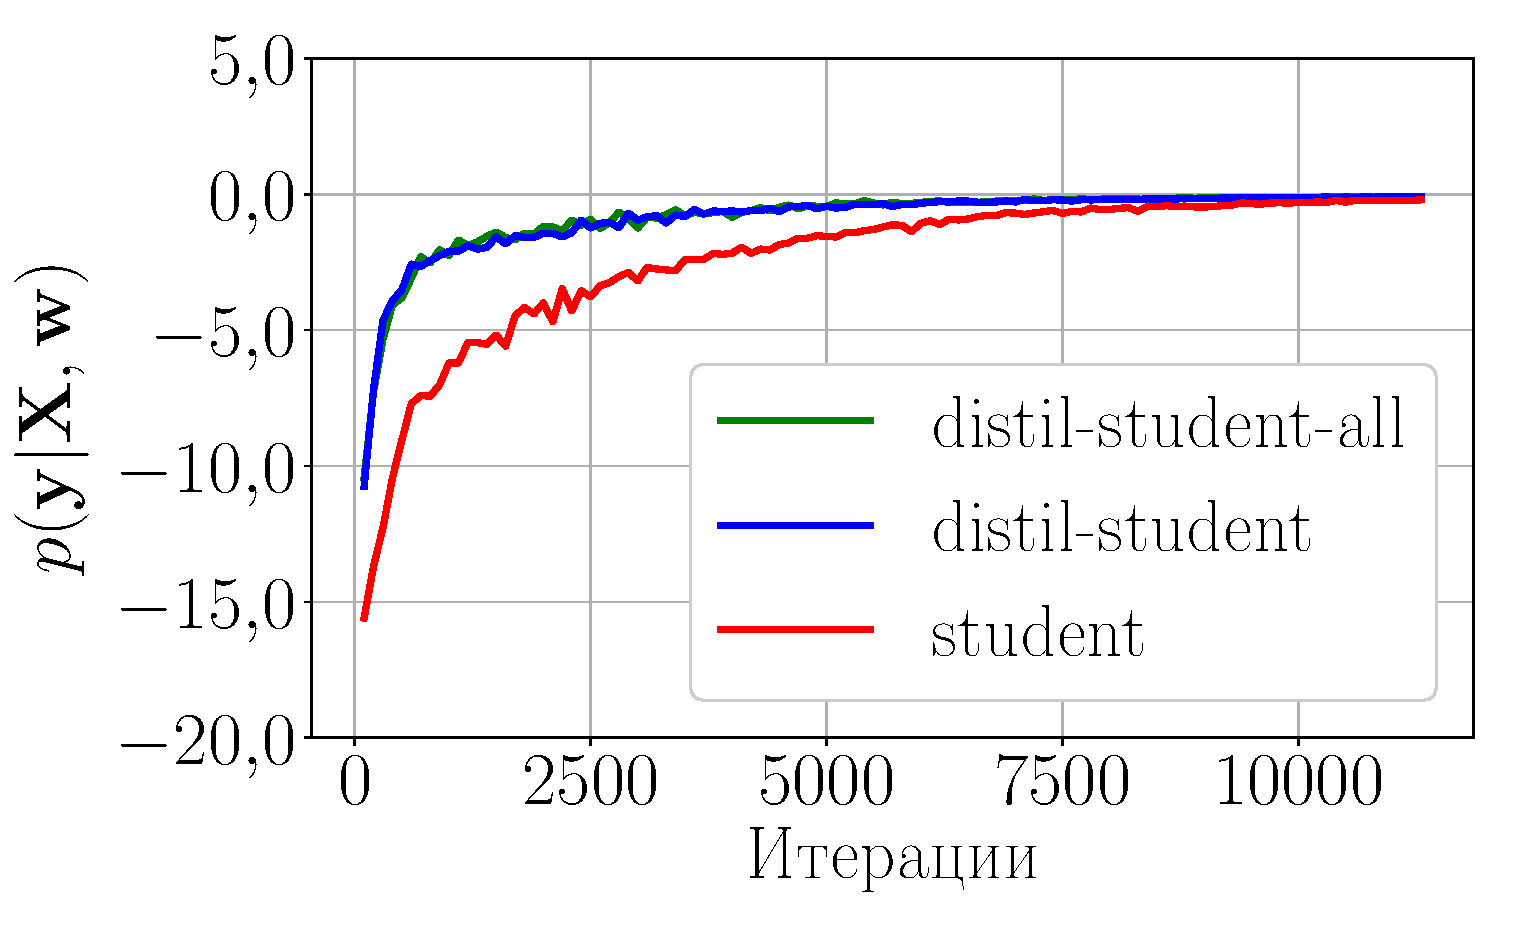
\includegraphics[width=0.5\textwidth]{synthetic_likelihood_3_layers.eps}
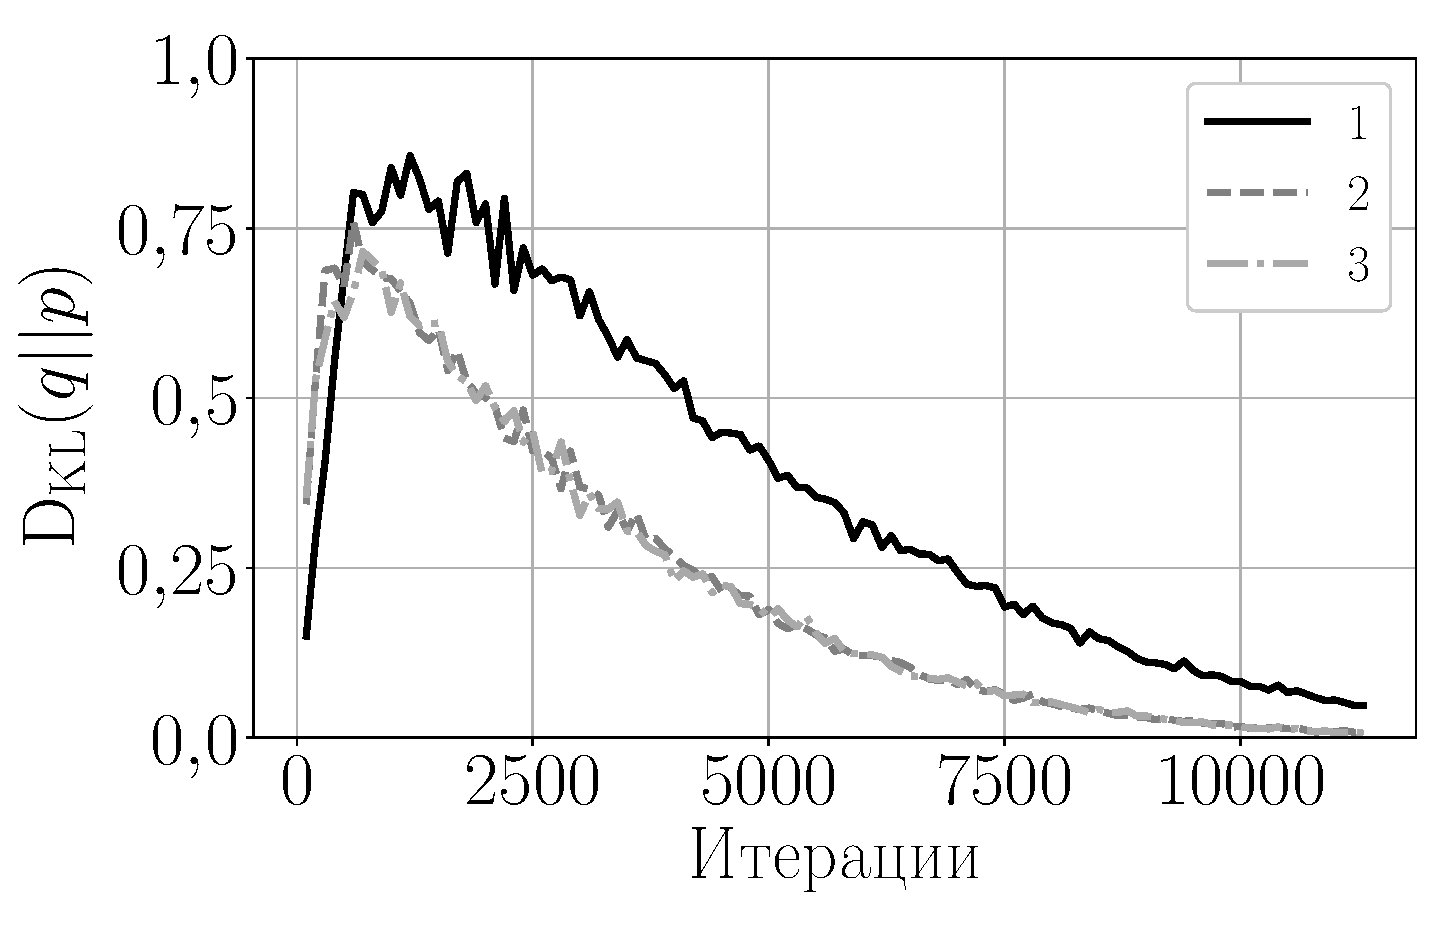
\includegraphics[width=0.5\textwidth]{synthetic_D_KL_3_layers.eps}
\caption{Рис. 1.}
\label{exp:fig1}
\end{figure}

\begin{figure}[h!]
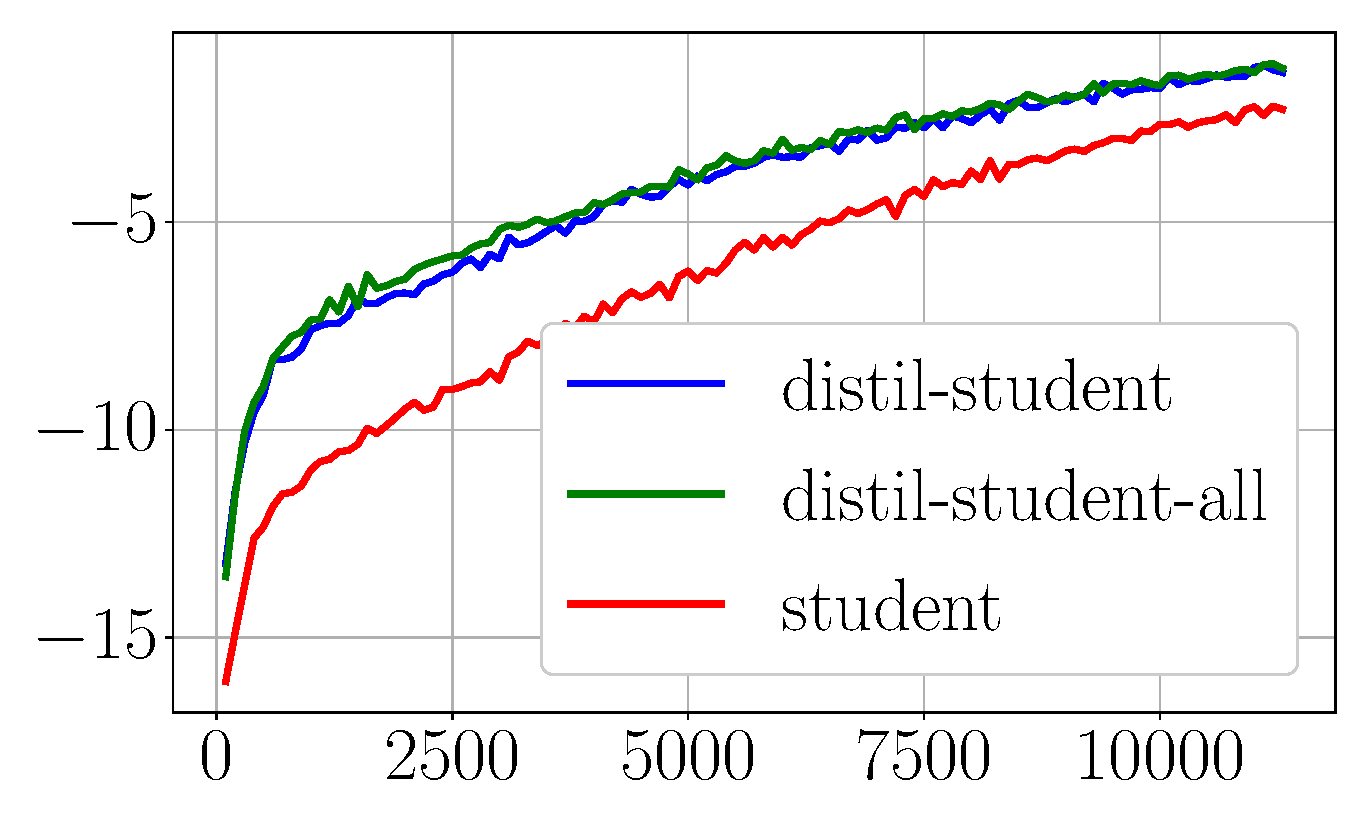
\includegraphics[width=0.5\textwidth]{synthetic_likelihood_2_layers.eps}
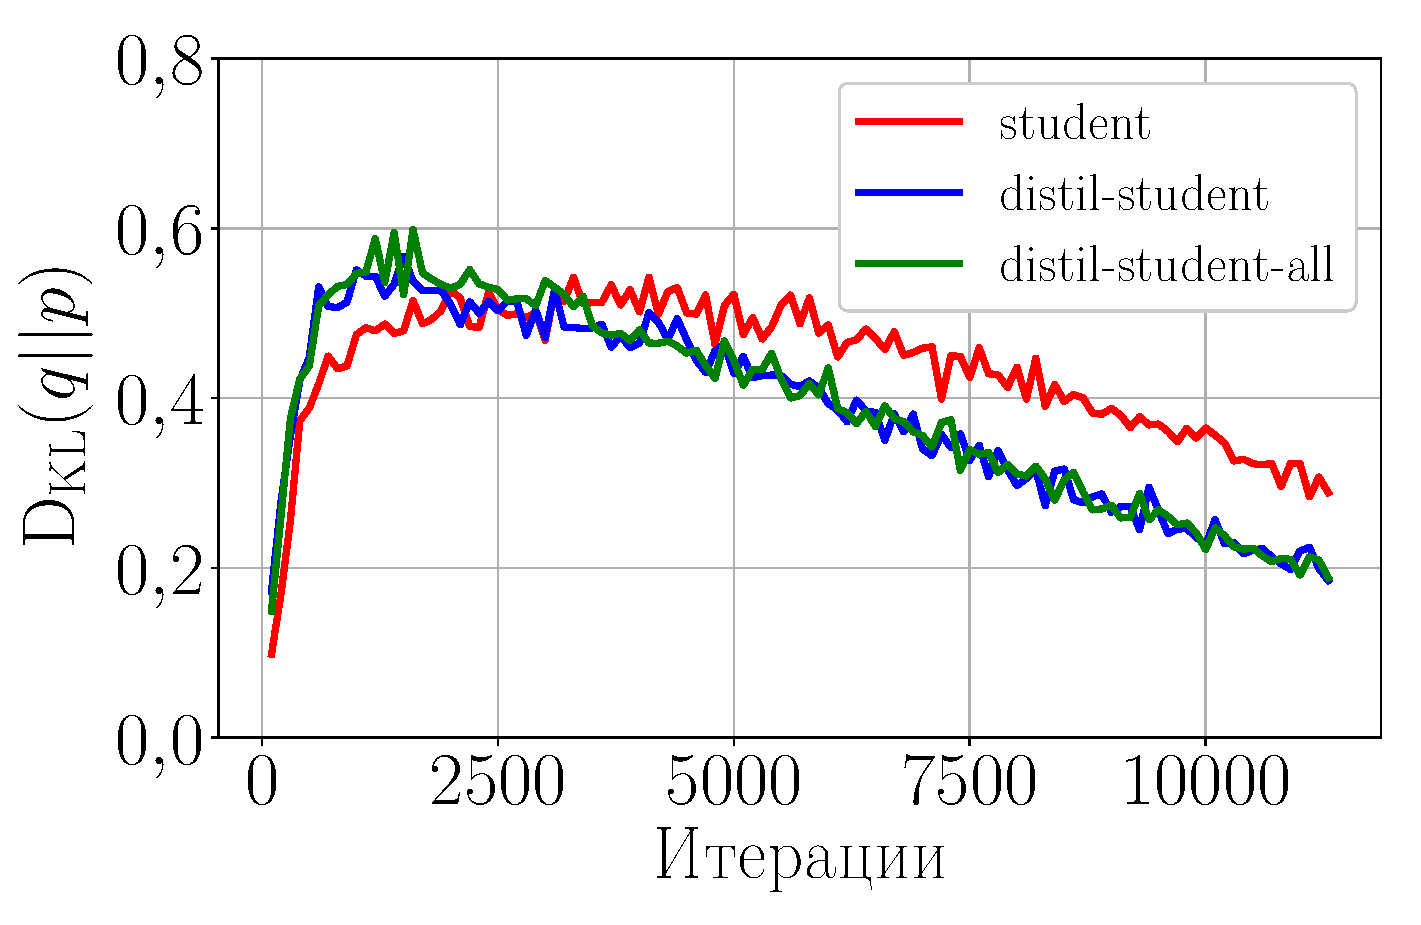
\includegraphics[width=0.5\textwidth]{synthetic_D_KL_2_layers.eps}
\caption{Рис. 2.}
\label{exp:fig2}
\end{figure}

\begin{figure}[h!]
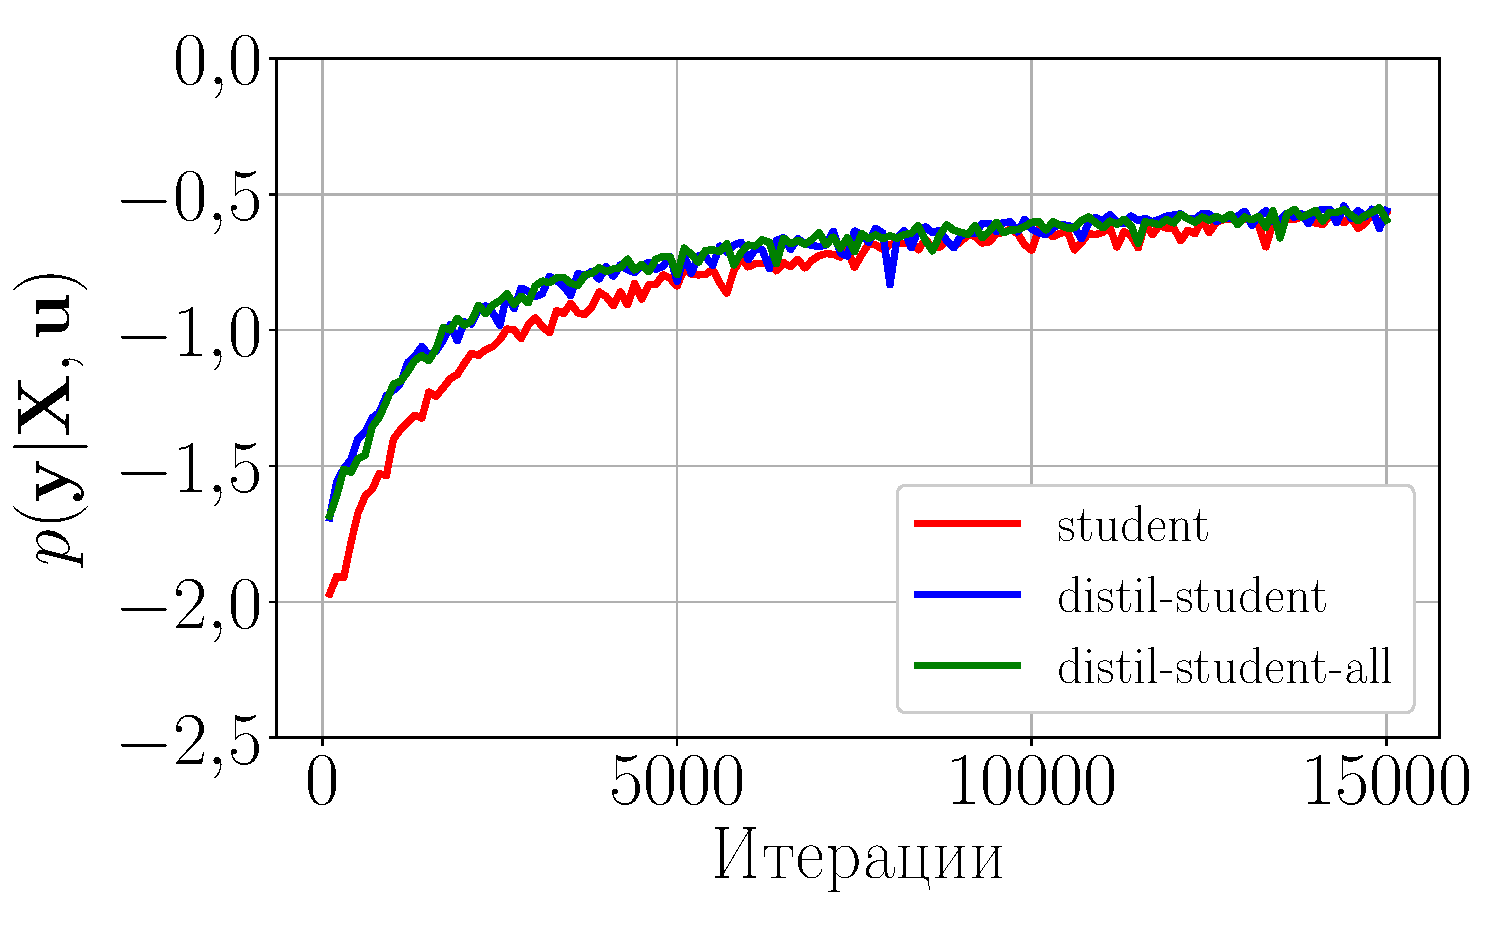
\includegraphics[width=0.5\textwidth]{fashionmnist_likelihood_2_layers.eps}
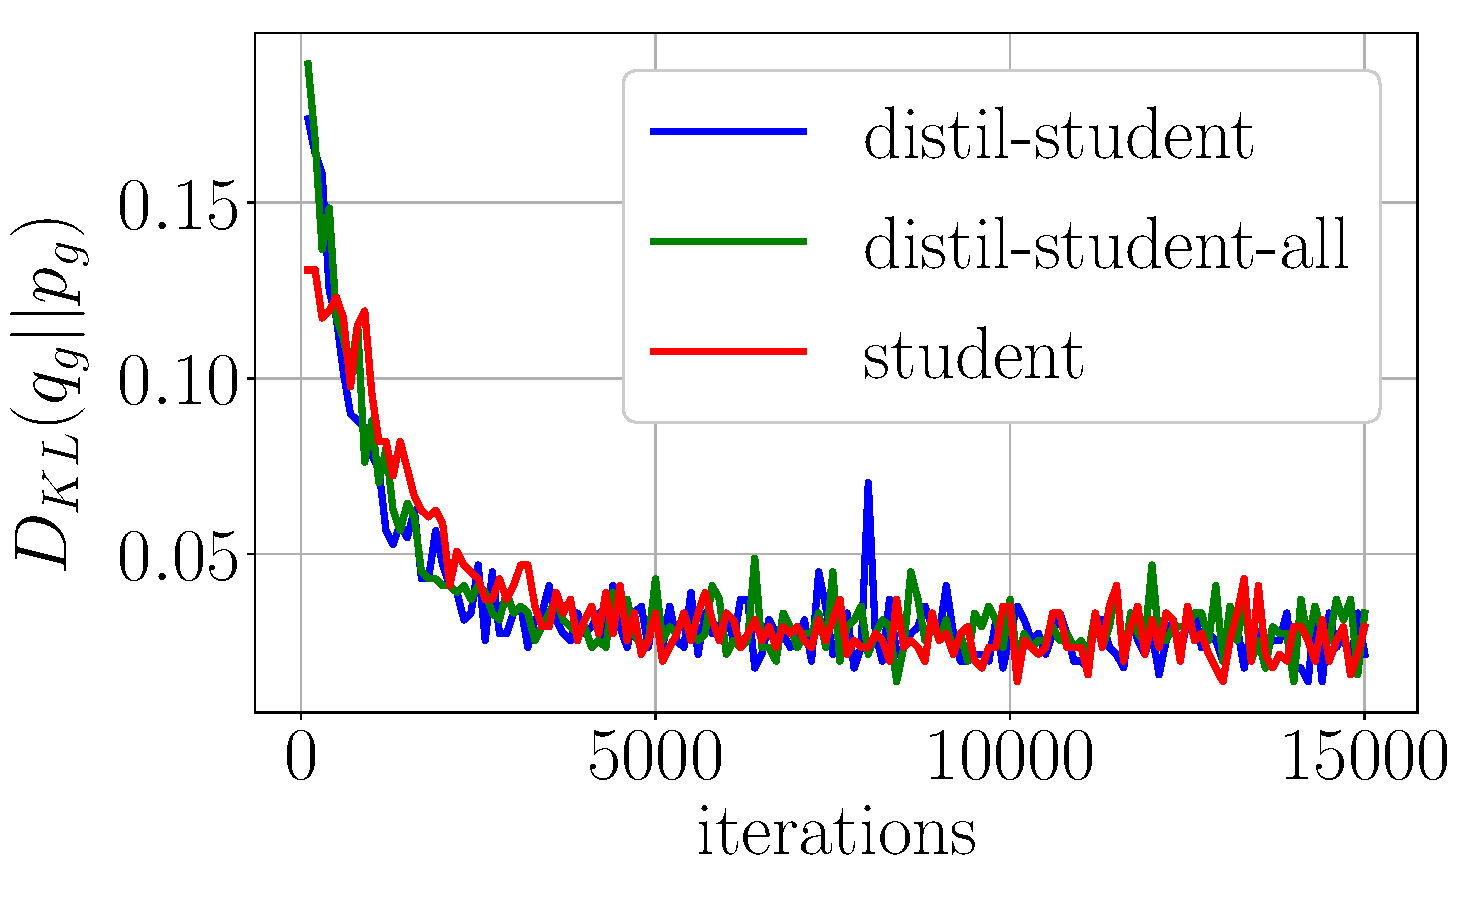
\includegraphics[width=0.5\textwidth]{fashionmnist_D_KL_2_layers.eps}
\caption{Рис. 3.}
\label{exp:fig3}
\end{figure}

\newpage
~\\
Рис.~1. Структура~\eqref{eq:ex:3} модели ученика $g$. Слева: правдоподобие выборки в зависимости от номера итерации при обучении. Справа: дивергенция Кульбака--Лейблера между вариационным и априорным распределениями параметров модели.
\\~\\
Рис.~2. Структура~\eqref{eq:ex:5} модели ученика~$g$. Слева: правдоподобие выборки в зависимости от номера итерации при обучении. Справа: дивергенция Кульбака--Лейблера между вариационным и априорным распределениями параметров модели.
\\~\\
Рис.~3. Слева: правдоподобие выборки в зависимости от номера итерации при обучении. Справа: дивергенция Кульбака--Лейблера между вариационным и априорным распределениями параметров модели.

\end{document}
